
{
\setlength{\tabcolsep}{5pt}
\begin{table}[!t]{
\centering
\begin{tabular}{rcc}
					&  {\bf Cori} & {\bf Edison }    \\
					& ({\bf Intel KNL})  & ({\bf Intel Ivy Bridge})		\\
\hline%----------------------------------------------------------------------------
{\bf Core }	 	 & 			& \\

\hline%----------------------------------------------------------------------------
Clock (GHz)			& 1.4			& 2.4					\\
L1 Cache (KB)		& 32		& 32				\\
L2 Cache (KB)		& 1024$^1$		& 256				\\
DP GFlop/s/core		& 44			&19.2		\\
\hline%----------------------------------------------------------------------------
{\bf Node Arch.}	 	 & 			& \\
\hline%----------------------------------------------------------------------------
Sockets/node			&  1		&	2					\\
Cores per socket			& 64				& 12					\\
STREAM BW$^2$		&  102~GB/s 	&	104~GB/s		\\
Memory per node		&  96~GB	&	64~GB			\\
\hline%-------------------------------------------------------------------------
{\bf Prog. Environment}	 	 & 			& \\
\hline%----------------------------------------------------------------------------
Compiler & gcc 5.3.0 & gcc 5.3.0\\
Optimization & -O3 &  -O3 \\
\hline%----------------------------------------------------------------------------
\end{tabular}

\caption{Overview of Evaluated Platforms.  $^1$Shared between 2 cores in a tile. $^2$Memory bandwidth is measured using the STREAM copy benchmark per node.}
\label{tab:machines}
}
\end{table}
}


%\begin{table*}[!ht]
% \centering
% \caption{Test problems from the University of Florida sparse matrix collection~\cite{davis2011university}. 
%}
%
% \begin{tabular}{@{} l l c  c   c   l @{}}
%    \toprule
%    
% Class & Graph	&	\#vertices	&	\#edges &	 pseudo & Description\\
% & &	($\times 10^6$)	&	($\times 10^6$) 	&	diameter  &	\\
%
%  \toprule
%%\multirow{6}{*}{\begin{sideways}Square\end{sideways}}  
%& amazon0312	&	0.40	&	3.20			& 21	&	Amazon product co-purchasing network	\\
%& web-Google	&	0.92	&	5.11			&	16	&	Webgraph from the Google prog. contest, 2002	\\
%low-diameter graphs  &  	wikipedia-20070206	&	3.56	&		45.03	&	14	&	Wikipedia page links	\\
% & ljournal-2008	&	5.36	&		79.02 & 34	&	LiveJournal social network\\
%  &  wb-edu	&	9.85	&	57.16	&	38	&	Web crawl on .edu domain	\\
%    &  dielFilterV3real	&	1.10	&		89.31	&	84 &		High-order vector finite element method in EM\\ 	
%
%
%  \midrule 
%  &  G3\_circuit	&	1.56	&	7.66	&	514 &		circuit simulation problem	\\ 
%   &   hugetric-00020	&	7.12		&	21.36		&	3,662 &		undirected graph\\	
%  high-diameter graphs&   hugetrace-00020	&	16.00		&	48.00		&	5,633 &		Frames from 2D Dynamic Simulations\\
% &  delaunay\_n24	&	16.77		&	100.66	& 1,718	&		Delaunay triangulations of random points\\ 
%
% & rgg\_n24\_s0	&	16.77	&	165.1	&	3,069  &	Random geometric graph\\ 
%
%  	       \toprule
%  \end{tabular}
%\label{table:problem-statistics}
% \end{table*}



\section{Results}
\label{sec:results}

\subsection{Experimental Setup} 
We evaluate the performance of LACC on NERSC/Edison and NERSC/Cori (KNL) systems  as described in Table~\ref{tab:machines}.
We used OpenMP for multithreaded execution in our code. 
In our experiments, we only used square process grids because rectangular grids are not supported in CombBLAS~\cite{bulucc2011combinatorial}. 
When $p$ cores are allocated for an experiment, we create a $\sqrt{p/t} \times \sqrt{p/t} $ process grid where $t$ is the number of threads per process.
Unless otherwise stated, all of our experiments on Cori used 16 threads per MPI process.
In our hybrid OpenMP-MPI implementation, all MPI processes perform local computation followed by synchronized communication rounds. 
Local computation in every matrix-algebraic kernel is fully multithreaded using OpenMP.
Only one thread in every process makes MPI calls in the communication rounds (that is \texttt{MPI\_THREAD\_FUNNELED} thread support is used in \texttt{MPI\_Init\_thread} function call).
%The source code of the distributed-memory MCM algorithm is publicly available as part of Combinatorial BLAS library~\cite{CombBLAS1.5}.


 %Table~\ref{table:problem-statistics} describes a set of real matrices from the University of Florida sparse matrix collection~\cite{davis2011university} used in our experiments.
 %We selected the low-diameter scale-free graphs and high-diameter graphs arising in various scientific domains.
% To test the performance of our matching algorithm on larger matrices,  we used RMAT~\cite{rmat}, the Recursive MATrix generator to generate three different classes of synthetic matrices: (a) G500 matrices  representing graphs with skewed degree distributions from Graph 500 benchmark~\cite{graph500}, (b) SSCA matrices from HPCS Scalable Synthetic Compact Applications graph analysis (SSCA\#2) benchmark~\cite{SSCA}, and (c)  ER matrices representing \erdosrenyi~ with uniform degree distributions.
%We use the following RMAT seed parameters to generate these matrices: (a) $a{=}.57$, $b{=}c{=}.19$, and $d{=}.05$ for G500, (b) $a{=}.6$, and $b{=}c{=}d{=}.4/3$ for SSCA, and (c) $a{=}b{=}c{=}d{=}.25$ for ER.
%A scale $n$ synthetic matrix is $2^n$-by-$2^n$.
%On average, G500 and ER matrices have $32$ nonzeros, and SSCA matrices have $16$ nonzeros per row and column.
%%We compactly describe a synthetic graph, by its "scale``  where a graph has $2^{scale}$ vertices.
%For example, a scale-30 G500 matrix (\texttt{G500-30}) has about 1 billion rows, 1 billion columns, and 32 billion nonzeros.  
%We applied a random permutation to the input matrices to balance the memory and the computational load.
%%Let $A$ be an $m\times n$ matrix with $\id{nnz}$ nonzero entries.
%%We consider the matrix representing an undirected bipartite graph $G(R\cup C, E)$ where every row (column) of $A$ is represented by a vertex in $R$ ($C$), and each nonzero entry $A[i,j]$ of $A$ is represented by two edges $(r_i,c_j)$ and $(c_j,r_i)$ connecting the $i$th row and $j$th column vertices.	
%









\subsection{Impact of sorted input and output vectors on the performance of the SpMSpV-bucket algorithm}
We implemented two variants of the SpMSpV-bucket algorithm based on the sortedness of the input and output vectors: in one variant both $\mathbf{x}$ and $\mathbf{y}$ are kept sorted by their indices, while the second variant works on unsorted vectors.
Figure~\ref{fig:sorting} shows the impact of sorted vectors on the performance of the SpMSpV-bucket algorithm for $\mathbf{x}$ with 10K and 2.5M nonzeros.
When the vector is relatively dense, keeping the vectors sorted improves the performance of our algorithm as can be seen in the right subfigure in  Figure~\ref{fig:sorting}.
This is due to the fact that when $\mathbf{x}$ is denser, the probability of accessing consecutive columns of $\mA$ increases, making the bucketing step (Step 1 in Algorithm 1) more cache efficient.
By contrast, columns of  $\mA$ are often accessed inconsecutively when $\mathbf{x}$ is sparser (e.g., when $\dnnz(\mathbf{x})$ is less than $1\%$ of $n$).
Since the unsorted version never seems to outperform the sorted version in practice, we only present results with sorted vectors in the remainder of the results section.
Sorted vectors also ensure fairness when comparing our algorithm with existing algorithms (GraphMat and CombBLAS) that keep their vectors ordered. 


\begin{figure}[!t]
   \centering
   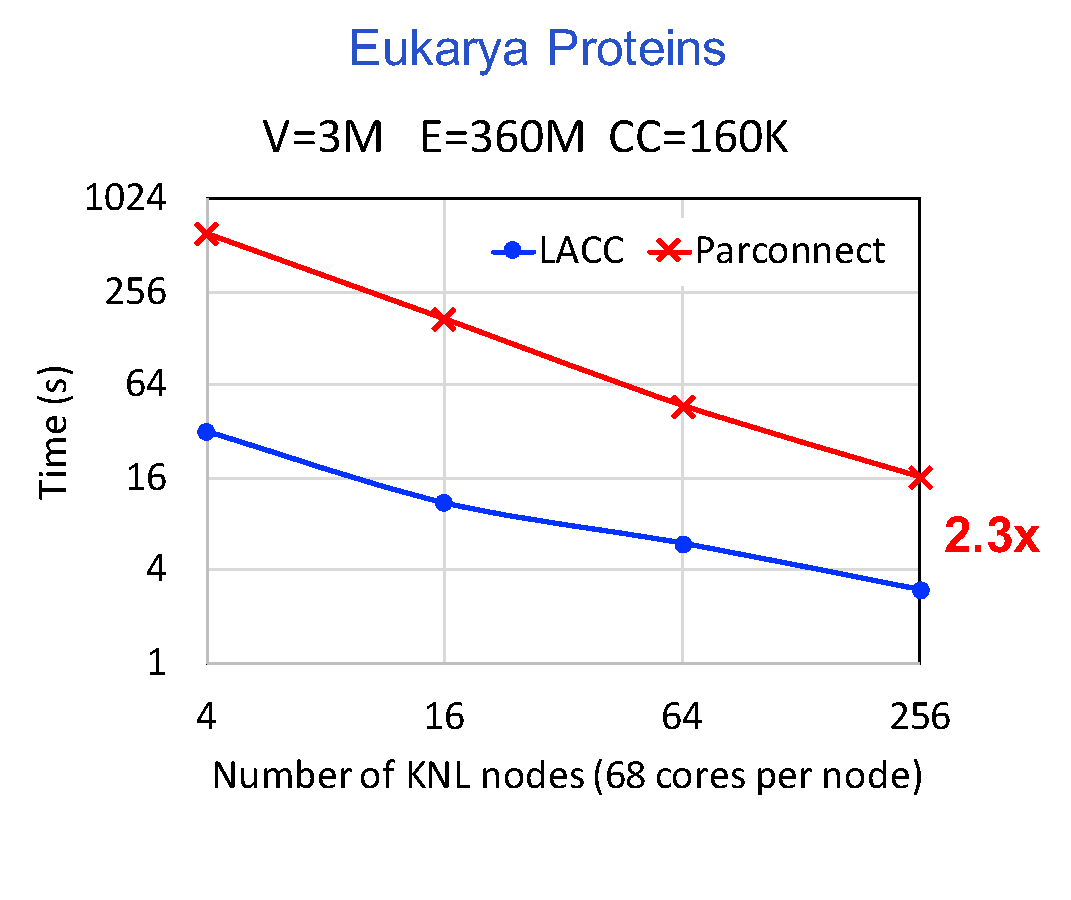
\includegraphics[scale=.5]{figures/eukarya} % requires the graphicx package
   \caption{Strong scaling of LACC and Parconnect when finding connected components in  the eukarya protein similarity network. }
   \label{fig:sorting}
\end{figure}

\begin{figure}[!t]
   \centering
   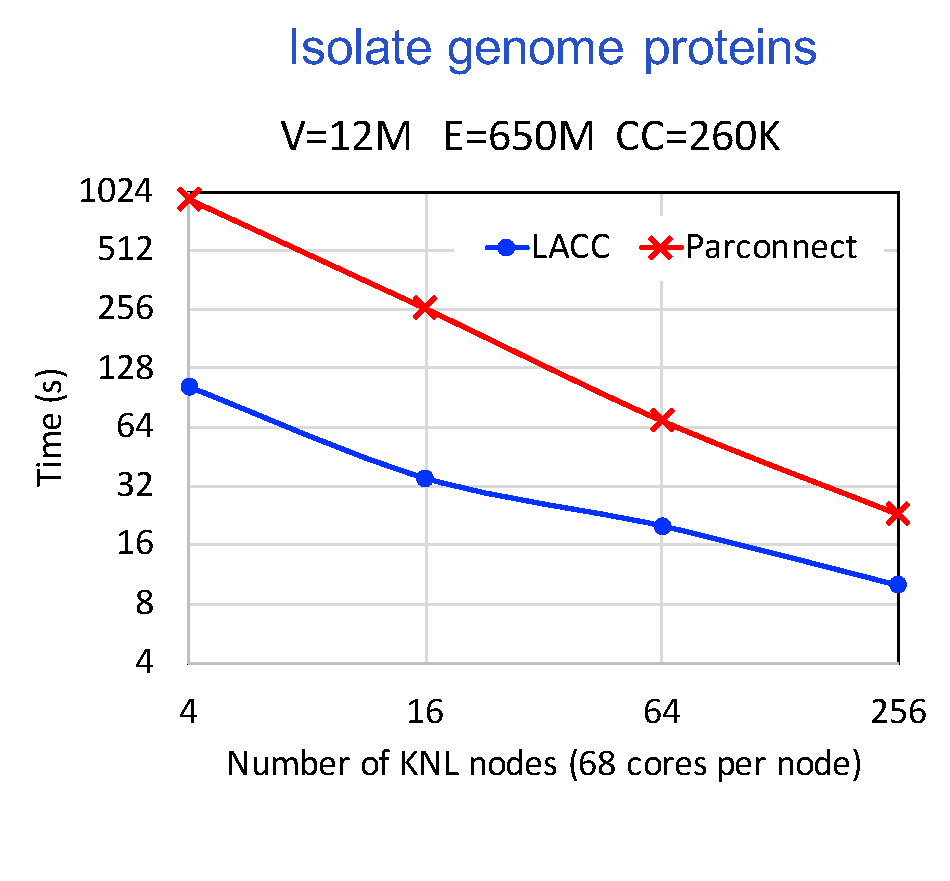
\includegraphics[scale=.5]{figures/isolates} % requires the graphicx package
   \caption{Strong scaling of LACC and Parconnect when finding connected components in  the isolate genomes protein similarity network. }
   \label{fig:multiply_nnzx}
\end{figure}

\begin{figure*}[!t]
   \centering
   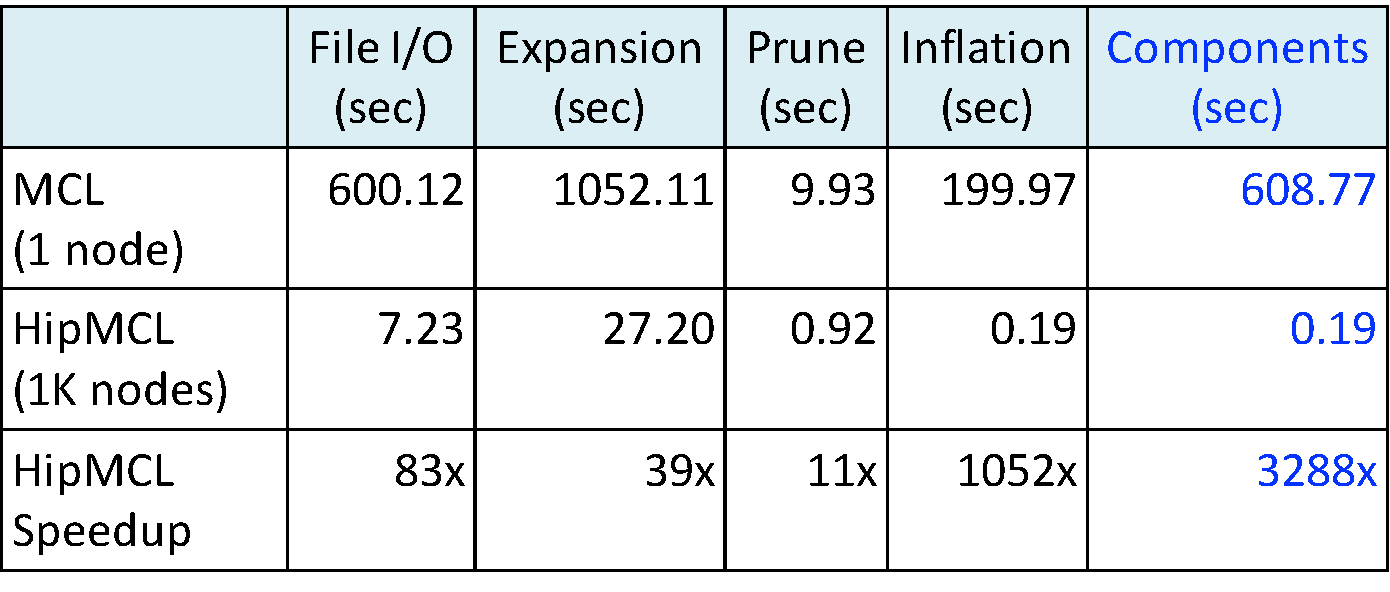
\includegraphics[scale=.5]{figures/hipmcl} % requires the graphicx package
   \caption{Performance improvement by LACC when used in HipMCL over the default shared-memory CC algorithm used in MCL. This result is obtained when clustering eukaryotic network with 3 million nodes and 359 million edges on NERSC/Edison.}
   \label{fig:hipmcl}
\end{figure*}




